%%%%%%%%%%%%%%%%%%%%%%%%%%%%%%%%%%%%%%%%%%%%%%%%%%%%%%%%%%%%%%%%%%%%%%%%%%%%%%%%
% Limit_Intepretation.tex: Select of showering and tracking events:
%%%%%%%%%%%%%%%%%%%%%%%%%%%%%%%%%%%%%%%%%%%%%%%%%%%%%%%%%%%%%%%%%%%%%%%%%%%%%%%%
\chapter{Limit Interpretation}
\label{Limit_Results_and_Intepretation_Chapter}
%%%%%%%%%%%%%%%%%%%%%%%%%%%%%%%%%%%%%%%%%%%%%%%%%%%%%%%%%%%%%%%%%%%%%%%%%%%%%%%%
The observed~($N^{Obs}$) confidence limit on the number of events is related to the expected~($N^{Expt}$) number of events from the SPS8 GSMB model through the relation
\begin{equation}{\label{eq:NUPA}}
 \mu^{UL} = \frac {N^{Obs}}{N^{Expt}}
\end{equation}
where, $\mu^{UL}$, is the upper limit on the signal strength obtained from running the HiggsCombine tool  with the $CL_{s}$ procedure.
Using the relationship between the cross section~($\sigma$) and the number of events~($N$): $\sigma = \frac{N}{\varepsilon\times A \cdot \mathscr{L}}$, and Equation \ref{eq:NUPA}, the observed upper limit on the cross section is evaluated in the following way:
\begin{equation}{\label{eq:SIGMAUPA}}
\sigma^{Obs}_{UL} = \frac{\mu^{UL} \cdot N^{Expt}}{\varepsilon\times A\cdot \mathscr{L}}
\end{equation}
where, $\mathscr{L}$, is the integrated luminosity~(19\fbinv) and $\varepsilon$ and $A$ are the signal selection Efficiency and Acceptance, respectively.
\par 
In addition to the \textbf{observed} limit~(shown as a solid black line in Figure \ref{fig:SPS8_Ctau_Ulimit}), we also evaluate the uncertainties on the \textbf{expected} or median~(50\%) limit~(dashed red line) at 68\%~($+ 1\sigma$) or 16\%~($- 1\sigma$) and at 98\%~($+ 2\sigma$) or 2.5\%~($- 2\sigma$) shown with the \textcolor{green}{GREEN} and \textcolor{yellow}{YELLOW}  bands, respectively, in the same Figure \ref{fig:SPS8_Ctau_Ulimit}.
\newline
Using the cross section from theory~(shown as the blue line in Figure \ref{fig:SPS8_Ctau_Ulimit}, for example), the excluded region in the mean lifetime of the lightest neutralino according to the SPS8 benchmark GMSB model are the values of mean lifetime, $\tau$, for which the observed cross section is below the theory cross section, \ie a lower limit and an upper limit on $\tau$ is extracted for the corresponding points where the observed cross section and the theory cross section intersect.
An exclusion  upper limit on the mass or effective SUSY breaking scale, $\mathbf{\Lambda}$, is obtained from Figure \ref{fig:MASS-limits} at the point where the observed cross section~(solid black line) intersects with the expected~(blue line) cross section. 
\newline
Using  the upper limits in $\tau$ and mass of the lightest neutralino or effective SUSY breaking scale, $\mathbf{\Lambda}$, we produce a two dimensional exclusion limit in $\tau$ and $\mathbf{\Lambda}$ and also a cross section limit according to the SPS8 benchmark GMSB model. 

%%%%%%%%%%%%%%%%%%%%%%%%%%%%%%%%%%%%%%%%%%%%%%%%%%%%%%%%%%%%%%%%%
\section{Signal Efficiency and Acceptance}
%%%%%%%%%%%%%%%%%%%%%%%%%%%%%%%%%%%%%%%%%%%%%%%%%%%%%%%%%%%%%%%%%
The plot in Figure \ref{fig:EffAcc} show our signal selection efficiency and acceptance for signal events of MC samples with different mean lifetime in \mm or \textit{proper decay length}, $c\tau$, ranging from 500\mm to 6000\mm with the same lightest neutralino mass of 255\GeVcc or effective SUSY breaking scale $\mathbf{\Lambda=180}$\TeV. 

\vspace{5mm}
\begin{minipage}{0.90\linewidth} 
\begin{center}
%\mbox{
%\includegraphics[width=0.49\textwidth,height=0.5\textwidth]
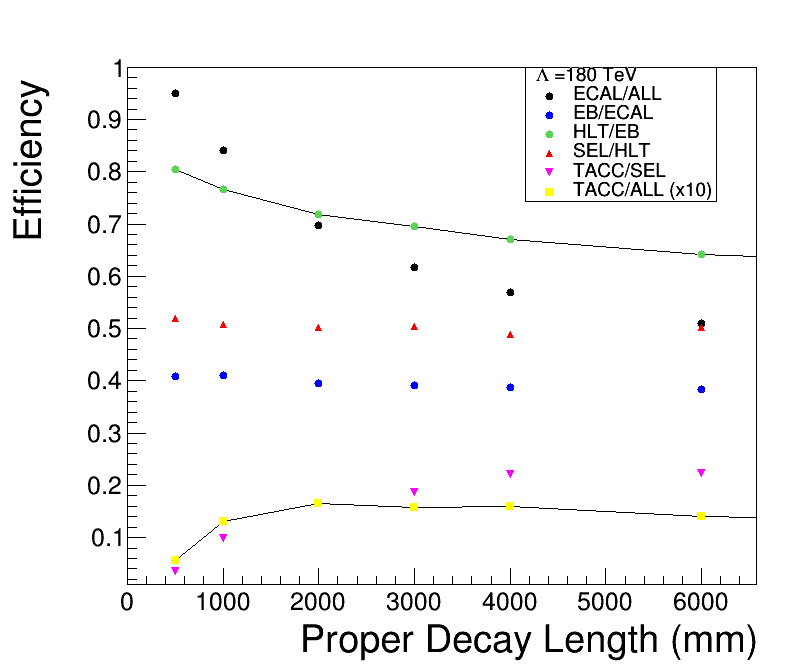
\includegraphics[height=0.65\textwidth, width=0.8\textwidth]{THESISPLOTS/Eff_180_ctau_2015.png}
%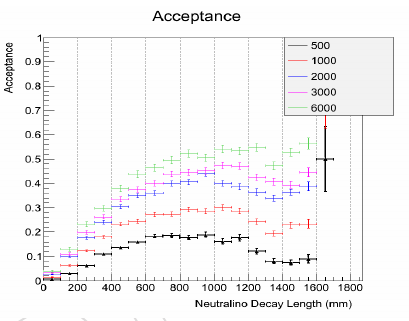
\includegraphics[height=0.5\textwidth, width=0.5\textwidth]{THESISPLOTS/SignalReconstructionAcceptance.png}}
\captionof{figure}{The efficiency for different mean decay length, $c\tau$~[\mm] with  $\mathbf{\Lambda=180}$\TeV. TACC/ALL~(yellow square markers) is the  Efficiency $\times$ Acceptance($t>3$~ns) \ie $\varepsilon \times A$, used in evaluating the exclusion limits. }
\label{fig:EffAcc}
\end{center}
\end{minipage}

\vspace{5mm}
The efficiency times acceptance~($\varepsilon \times A$) used in Equation \ref{eq:SIGMAUPA} to evaluate the exclusion limits is the TACC/ALL which is the ratio of the events passing our event selection with photon time, $t > 3$~ns in the barrel to all events with photons from the decay of the generated lightest neutralino. The $\times 10$  factor for TACC/ALL shown on the plot  is only for display purpose and was not used in evaluating the limits. 
\newline
The efficiency times acceptance, is small~(less than 10\%) for smaller values of $c\tau = 500\mm$~($\tau = 1.7$~ns) since very few of the events with photon from the lightest neutralino decay have time, $t > 3$~ns, despite many of photons reaching ECAL as is seen in the ECAL/ALL~(ratio of events with photons reaching ECAL to all events with photons from the decay of the generated lightest neutralino.) where the efficiency times acceptance is high for low $c\tau$ values. 
\newline
The efficiency times acceptance shown in Figure \ref{fig:EffAcc} peaks at $c\tau = 2000\mm$~($\tau = 6.7$~ns) and then begins to slightly fall for larger $c\tau$ values. For very large $c\tau > 6000\mm$ values not shown on the plots, the efficiency times acceptance is again less than 10\% since most of the lightest neutralinos decay outside of the ECAL and are undetected, as seen in the ECAL/ALL where the efficiency keeps dropping with increased $c\tau$ values.

\section{Systematic Studies}
We have required in our event selection that the photon \pt is greater than 80\GeVc, the jet \pt is greater than 35\GeVc and the missing energy is greater than 60\GeV. The same selection requirements applied to our MC signal event sample should guarantee a good event selection efficiency estimate. Any difference in the photon \pt, jet \pt and missing transverse energy between MC and data, will be a source of systematic uncertainties on the efficiency of selecting signal events. These uncertainties can come from quantities like jet energy scale~(JES), jet energy resolution~(JER), electron-photon energy scale, instrumentation related and energy deposits not clustered during missing transverse energy reconstruction, photon ECAL arrival time bias and ECAL time resolution. 
\newline
Table \ref{tab:SYST} presents the sources of uncertainties considered in this analysis. These uncertainties are computed by varying the nominal values of each quantity, while keeping the others fixed, by $1\sigma$ deviation and counting the number of events passing our event selection requirements. ECAL timing bias which has to do with the absolute reference time~(zero ns) of the ECAL timing, is the source of our largest uncertainty. The photon arrival time is measured with respect to this reference time. This ECAL time uncertainty has the largest impact on our analysis, since our analysis is based on counting the number of events with photon ECAL time above $3$~ns. The next largest uncertainties are from energy deposits missed by the clustering algorithm. This affects the photon energy scale, missing energy scale,  jet energy scale and resolution.
The uncertainty on the photon energy scale in the barrel was estimated to be 4.0\%  which is based on measuring the photon energy of events with $Z\rightarrow \mu\mu\gamma$ decay, where the muon radiates a photon in a process known as the final-state radiation~(FSR) \cite{PES}.  
\newline
The uncertainty on the \MET resolution uses a conservative estimate from \MET measurements in QCD events \cite{METRES}, where the \MET uncertainty is calculated using the fraction of events passing an event selection based on \MET for varying thresholds of \MET. 
\newline
The uncertainty on the ECAL time resolution was obtained by comparing the mean time of photons of events from $\gamma +$ jet MC sample to events from data with photon ECAL time, $|t_{\gamma}| < 2$~ns. The difference is found to be of the order of 200~ps per event. 
\newline
Meanwhile, the systematic uncertainty on luminosity measurement has the recommended value of $2.2$\% provided by CMS and LHC luminosity measurements while the uncertainty from Parton Density Functions~(PDF) is evaluated using the re-weighting technique which uses the Master Equation of CTEQ65 model set described in \cite{PDF}.
\newline
Since our background estimation is data-driven, the systematic uncertainties do not impact our results in a significant way.
The statistical uncertainty in the \textsf{ABCD} background estimation method is our largest source of uncertainty in this analysis and we estimate it to vary upward by 223\% and downward by 51\%. This large background statistical uncertainty is because of the very low event yields. Our final result is affected by the signal selection efficiency only, despite the large background estimation uncertainty. These signal selection uncertainties are used as nuissance parameters in the calculation of the upper limit on the observed signal cross section~($\sigma_{UL}$).

\vspace{5mm}
\begin{minipage}{0.90\linewidth} 
\begin{center}
%\begin{table}[ht]
%\renewcommand\arraystretch{1.2}
\begin{tabular}{c c}
\toprule
\hline
\bfseries{Source} & \bfseries {Uncertainty(\%)}\\
\hline
\toprule
\texttt{ECAL absolute time }~(0.0~ns) & $<10.0$\% \\
\texttt{ECAL time resolution}~(0.5~ns) & $<5.0$\% \\
\texttt{Unclustered energy deposits} & $<9.0$\% \\
\texttt{Photon energy scale}  & $< 4.0$\% \\
\texttt{Jet energy scale}~(JES)  & $< 9.0$\% \\
\texttt{Jet energy resolution}~(JER) &$ <9.0$\% \\
\texttt{\MET resolution} & $ <2.8$\%  \\
\texttt{PDF uncertainty} & $< 1.70$\% \\
\hline
\toprule
\texttt{Background estimation uncertainty} &$51.0$\% to 223\% \\
\hline 
\texttt{Luminosity}~(4.5\%) & $< 2.2$\% \\
\hline
\bottomrule
\end{tabular}
\captionof{table}{Summary of systematic uncertainties for signal efficiency and background estimation in this analysis and applied to our final results.}
\label{tab:SYST}
%\end{table}
\end{center}
\end{minipage}

\clearpage

\section{Limits on SPS8 GMSB Model}
If the effective SUSY breaking scale is $\mathbf{\Lambda} = 180\TeV$ then the upper limit on the product of the lightest neutralino production cross section and branching ratio decay to a photon and gravitino channel, $\PSneutralinoOne \rightarrow \gamma + \tilde{G}$, according to the SPS8 benchmark GMSB model is, $\sigma\times BR = 12.05$~fb. The mean lifetime of the lightest neutralino $\tau_{\PSneutralinoOne}$, is either less than $3.2$~ns or larger than 19.87~ns as shown in right plot of Figure \ref{fig:SPS8_Ctau_Ulimit}.

\vspace{5mm}
\begin{minipage}{0.90\linewidth}
\begin{center}
%\mbox{
%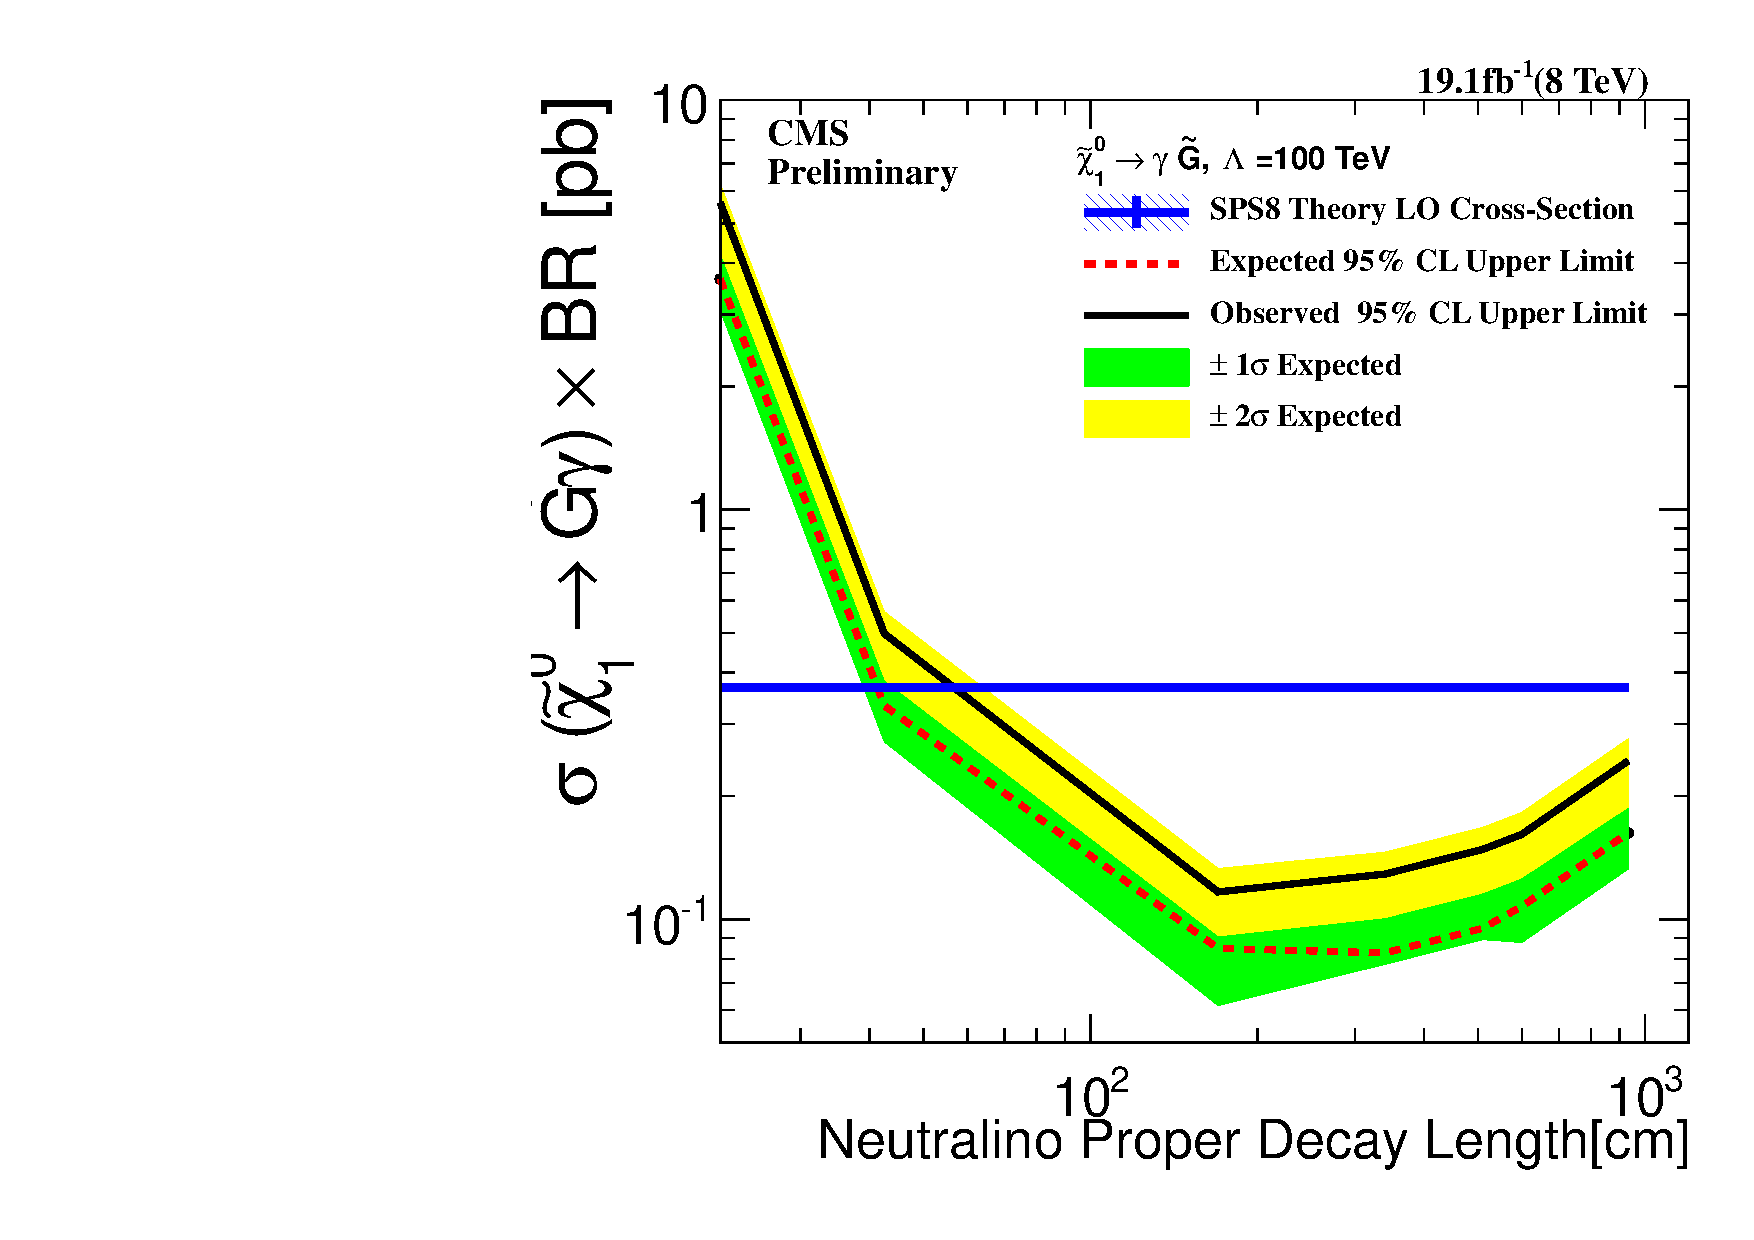
\includegraphics[height=0.65\textwidth, width=0.53\textwidth]{THESISPLOTS/100TeV_Neutralino_CrossSecTimesBR_Uplimit.pdf}
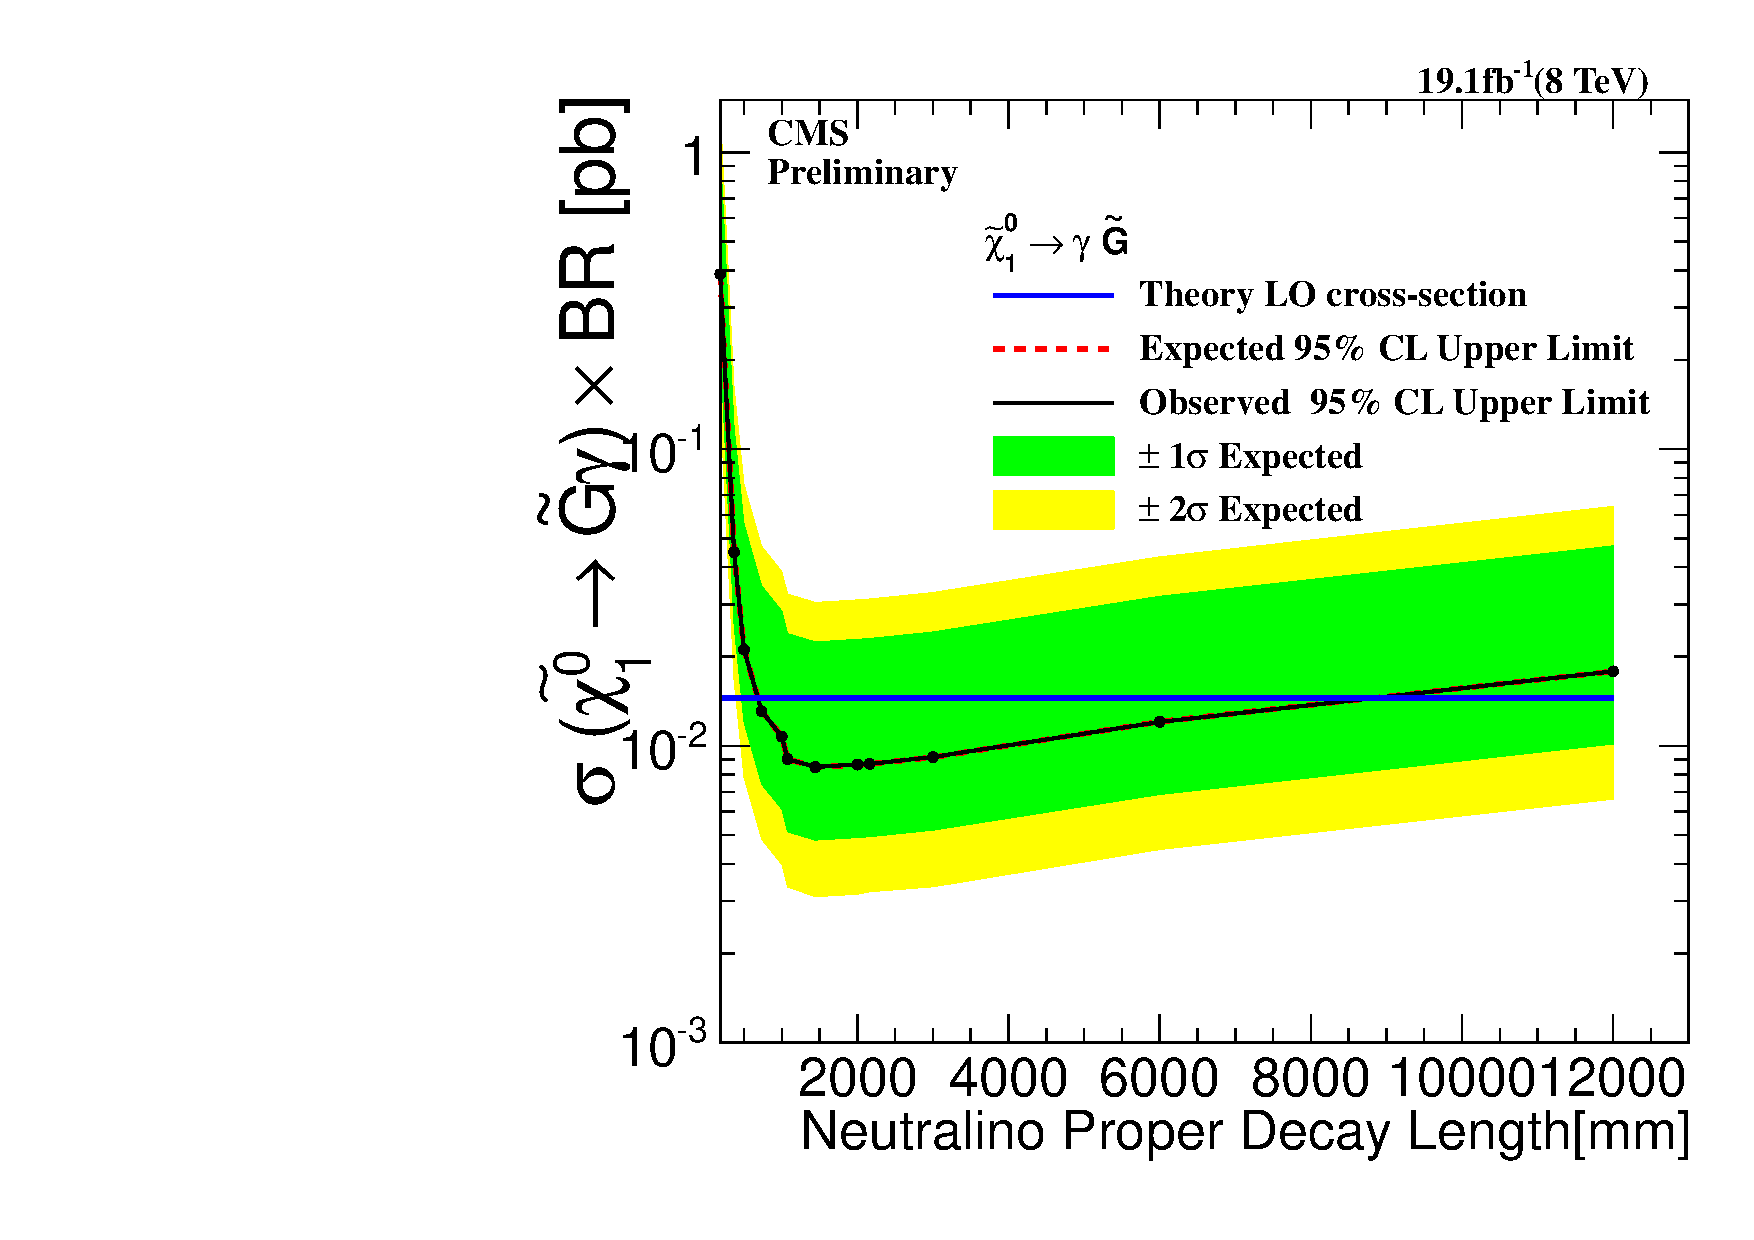
\includegraphics[height=0.8\textwidth, width=0.85\textwidth]{THESISPLOTS/Neutralino_CrossSecTimesBR_Uplimit.pdf} 
%}
\captionof{figure}{ 95\% CL evaluated using the $CL_{s}$ procedure on the lightest neutralino production cross section times branching ratio~($\sigma\times BR$) against mean lifetime~(ns) for $\mathbf{\Lambda = 180}$\TeV in the SPS8 benchmark GMSB model.}
\label{fig:SPS8_Ctau_Ulimit}
\end{center}
\end{minipage}
\vspace{5mm}

The excluded lightest neutralino mass, $m_{\PSneutralinoOne}$, or effective SUSY breaking scale, $\mathbf{\Lambda}$, observed from the cross section against lightest neutralino mass plot of Figure \ref{fig:MASS-limits} for $\tau = 6.7$~ns is up to  $m_{\PSneutralinoOne} = 300\GeVcc$ or  $\mathbf{\Lambda} = 220\TeV$, still in the context of the SPS8 benchmark GMSB model.
\newline
From the 2 dimensional plane define by $(\mathbf{\Lambda},\tau_{\PSneutralinoOne})$ of the exclusion limit, shown in  Figure \ref{fig:SPS8_2D-Ulimit}, the excluded lightest neutralino mean lifetime, $\tau_{\PSneutralinoOne}$, is from $2.0$~ns to $45.0$~ns for low mass~($m_{\PSneutralinoOne} < 150\GeVcc$) lightest neutralino. This exclusion in mean lifetime shrinks as the mass of the lightest neutralino increases or effective SUSY breaking scale increases. This is because the production cross section for the lightest neutralino decreases with increase in its mass or $\mathbf{\Lambda}$. 
\newline
For a given lightest neutralino mass and mean lifetime, we can also find its corresponding excluded cross section using Figure \ref{fig:SPS8_SIGMA-Ulimit}. For example, lightest neutralinos with mass,  $m_{\PSneutralinoOne} = 255\GeVcc$, or effective SUSY breaking scale,  $\mathbf{\Lambda} = 180\TeV$, and mean lifetime, $\tau_{\PSneutralinoOne} = 10.0$~ns, have an observed upper limit on their production cross section times branching ratio in the decay to photon and gravitino channel of $\sigma^{UP}_{\PSneutralinoOne} \geq 0.01$~pb at 95\% CL.

\vspace{5mm}
%\begin{figure}[!htb]
\begin{minipage}{0.90\linewidth}
%%\afterpage{ %
 %% \clearpage% Flush earlier floats (otherwise order might not be correct)
   %% \thispagestyle{empty}% empty page style (?)
%%\begin{landscape}% Landscape page
\begin{center}
%\mbox{
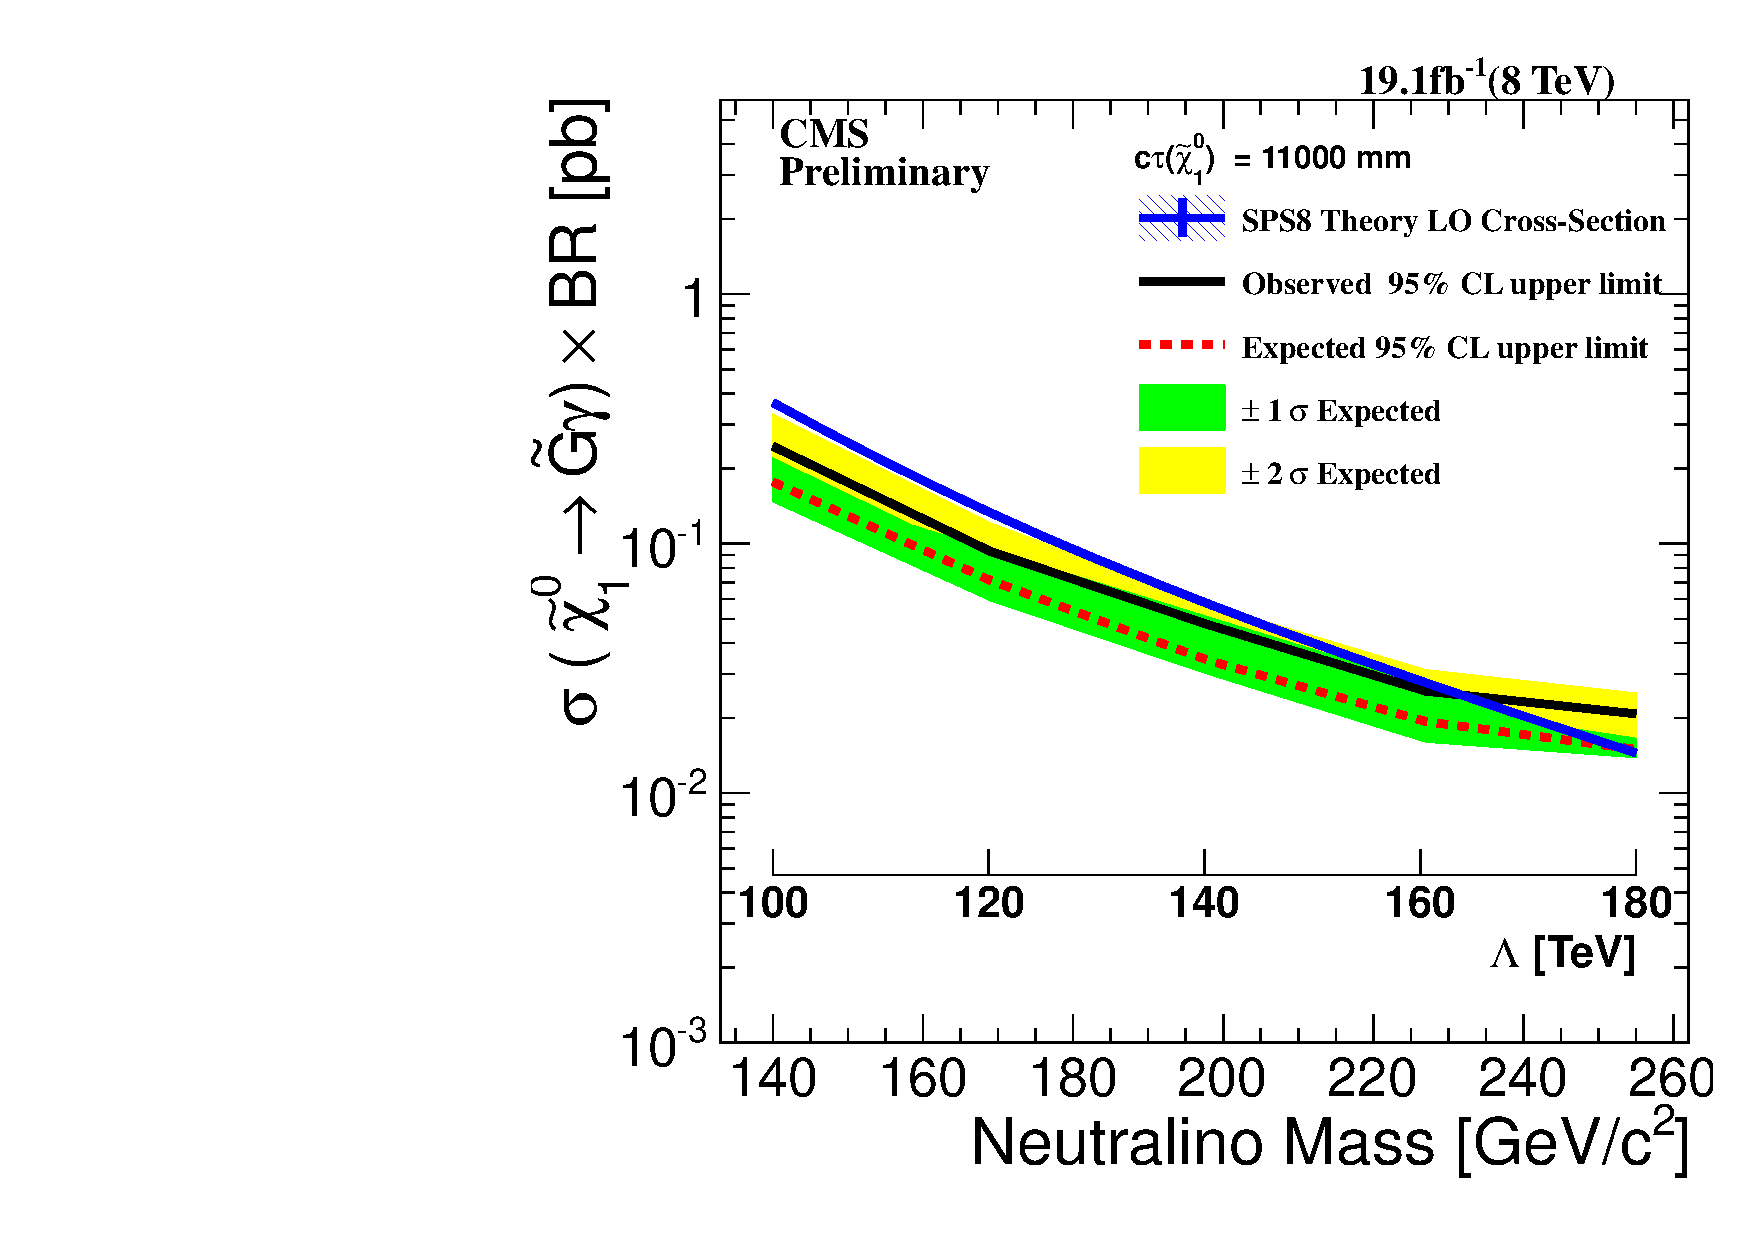
\includegraphics[height=0.8\textwidth, width=0.85\textwidth]{THESISPLOTS/Neutralino_CrosSecVsMass_Exclusion_limit_11000.pdf}
%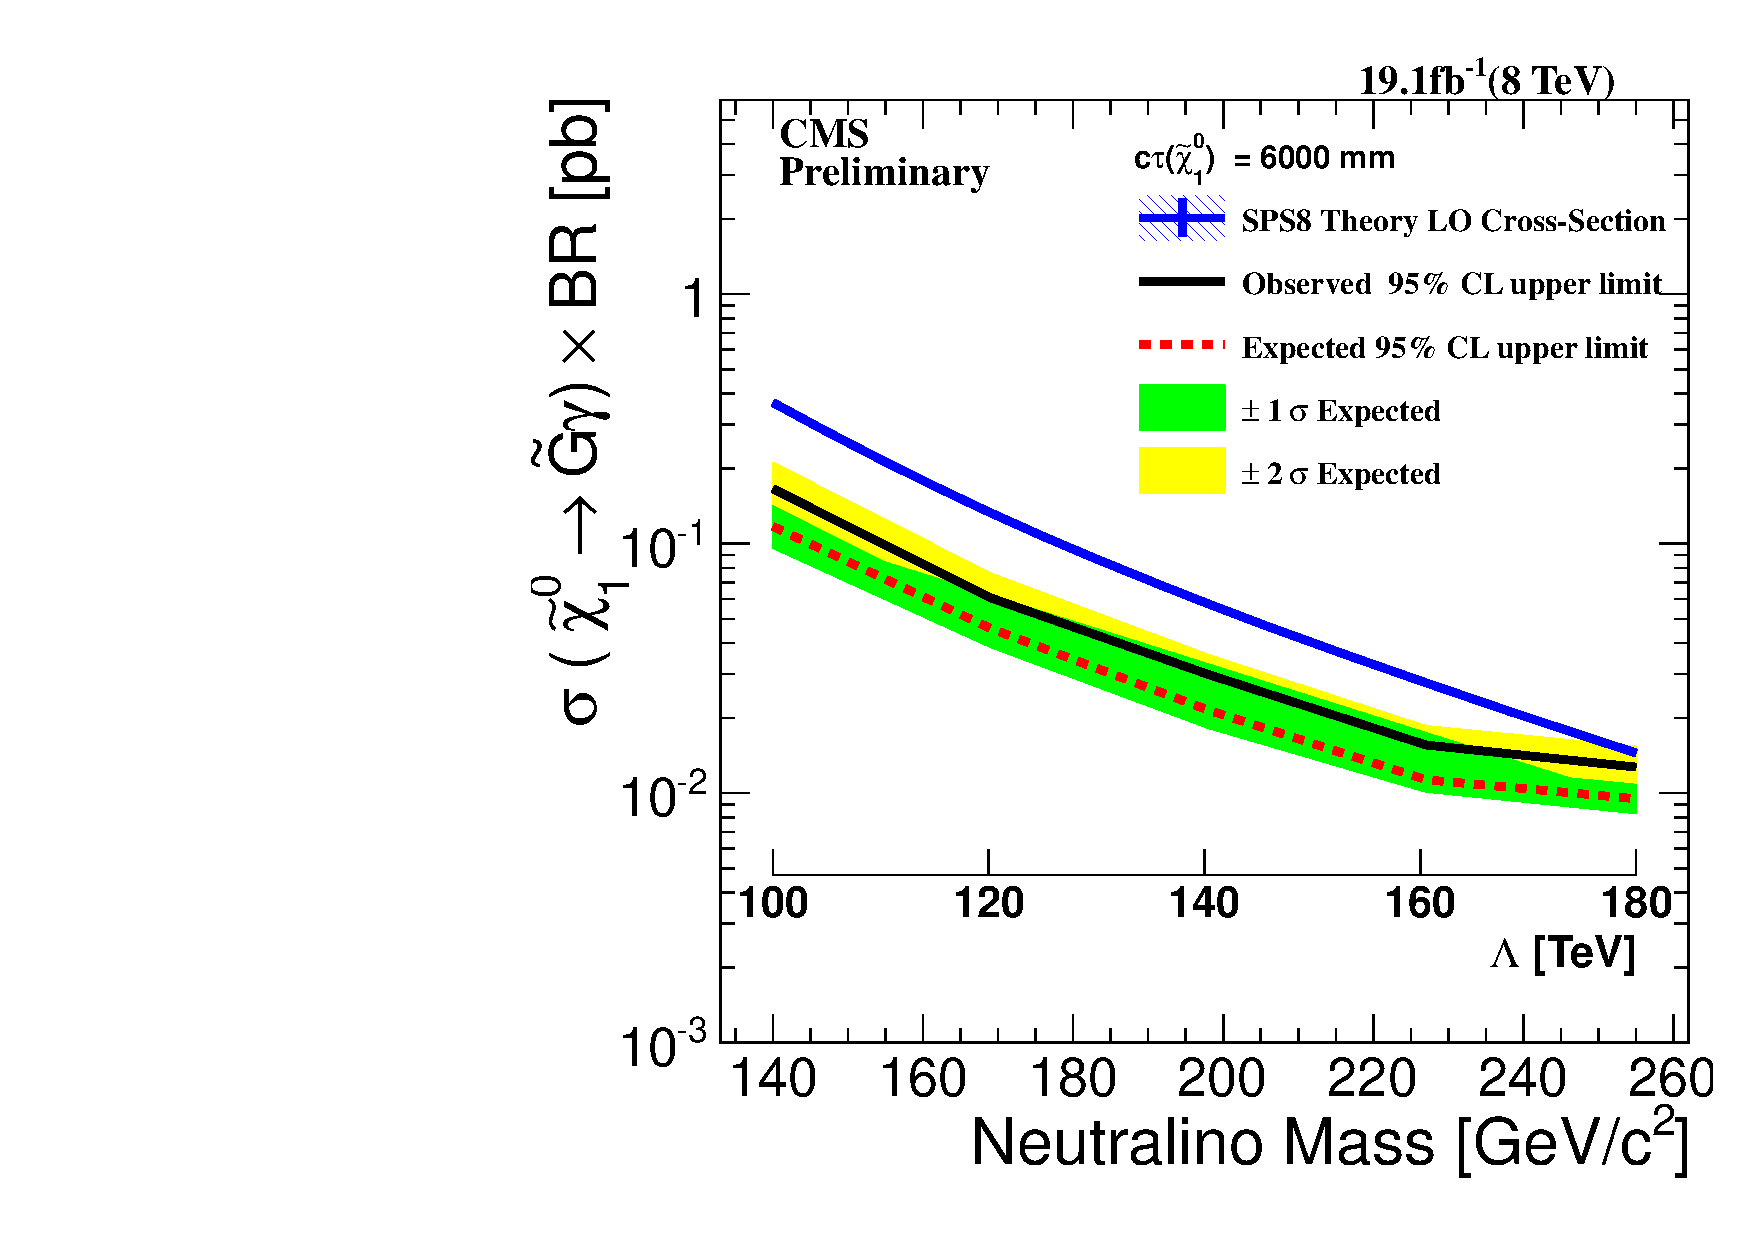
\includegraphics[height=0.65\textwidth, width=0.53\textwidth]{THESISPLOTS/Neutralino_CrosSecVsMass_Exclusion_limit_6000.pdf} }
\captionof{figure}{95\% CL evaluated using the $CL_{s}$ procedure on the lightest neutralino production cross section times branching ratio~($\sigma\times BR$) for different $\mathbf{\Lambda}$~(or mass of lightest neutralino) for $c\tau = 11000\mm$ or $\tau = 36.7$~ns in the SPS8 benchmark GMSB model.}
\label{fig:MASS-limits}
\end{center}
%\end{figure}
\end{minipage}
\vspace{5mm}

\begin{minipage}{0.95\linewidth}
\begin{center}
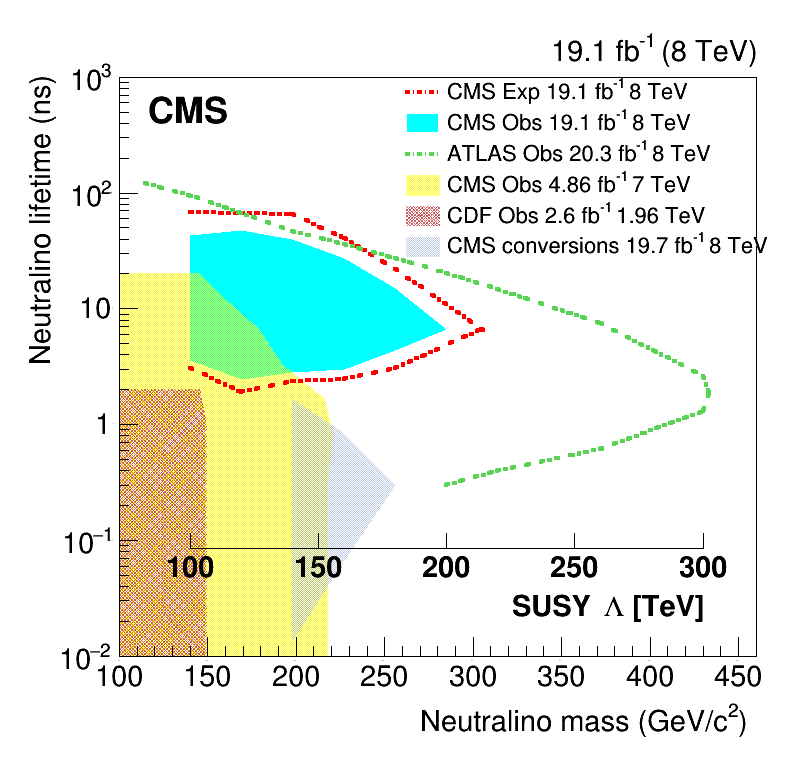
\includegraphics[height=0.85\textwidth, width=0.9\textwidth]{THESISPLOTS/Exclude2D_withAtlas_2015.png}
\captionof{figure}{95\% CL exclusion limit in lightest neutralino mass~(or $\mathbf{\Lambda}$) against mean lifetime in SPS8 benchmark GMSB model. Limits from previous experiments also shown.}
\label{fig:SPS8_2D-Ulimit}
\end{center}
\end{minipage}
\vspace{5mm}

\begin{minipage}{0.95\linewidth}
\begin{center}
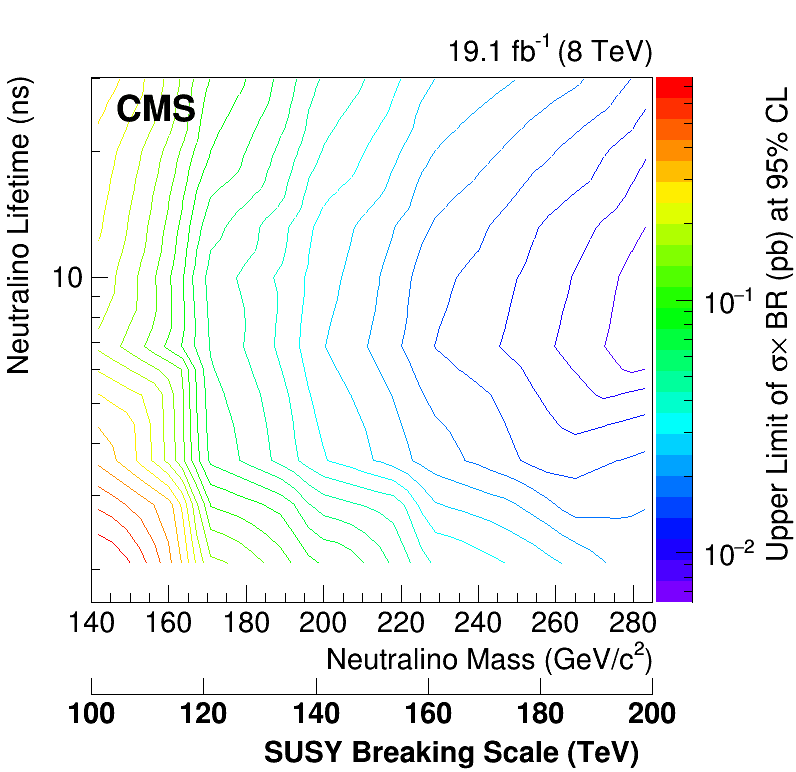
\includegraphics[height=0.85\textwidth, width=0.9\textwidth]{THESISPLOTS/limit2D_Cross-Section-Observed.png}
\captionof{figure}{95\% CL in cross section for different mass and lifetime of the lightest neutralino using the 8\TeV data corresponding to an integrated luminosity of 19.1\fbinv of the CMS experiment.}
\label{fig:SPS8_SIGMA-Ulimit}
\end{center}
\end{minipage}
%%\end{landscape}
%% \clearpage% Flush page
%%}

%%%%%%%%%%%%%%%%%%%%%%%%%%%%%%%%%%%%%%%%%%%%%%%%%%%%%%%%%%%%%%%%%%%%%%%%%%%%%%%%%%%%%%%%%%%%%%%%%%%%%%%
%%%%%%%%%%%%%%%%%%%%%%%%%%%%%%%%%%%%%%%%%%%%%%%%%%%%%%%%%%%%%%%%%%%%%%%%%%%%%%%%%%%%%%%%%%%%%%%%%%%%%%%

\begin{comment}
%%is given in table \ref{tab:SIGNALRES}
%%\vspace{5mm}
%%\begin{minipage}{\linewidth} 
%%\begin{center}
%\begin{table}[ht]
%\renewcommand\arraystretch{1.2}
%%\begin{tabular}{c c}
%%\toprule
%%\hline
%%\bfseries{SPS8 GMSB Signal} & \bfseries {Number of Events}\\
%%\hline
%%\toprule
%%\texttt{GMSB(SPS8)}~($\Lambda=180$~TeV,$c\tau=250$~mm) & $0.2096$ \\
%%\texttt{GMSB(SPS8)}~($\Lambda=180$~TeV,$c\tau=500$~mm) & $4.5423$  \\
%%\texttt{GMSB(SPS8)}~($\Lambda=180$~TeV,$c\tau=1000$~mm) & $6.3646$ \\
%%\texttt{GMSB(SPS8)}~($\Lambda=180$~TeV,$c\tau=2000$~mm) & $6.3968$ \\ 
%%\texttt{GMSB(SPS8)}~($\Lambda=180$~TeV,$c\tau=4000$~mm) & $6.1442$ \\
%%\texttt{GMSB(SPS8)}~($\Lambda=180$~TeV,$c\tau=6000$~mm) & $4.6498$ \\
%%\texttt{GMSB(SPS8)}~($\Lambda=180$~TeV,$c\tau=12000$~mm) & $2.918$ \\
%%\hline 
%%\bottomrule
%%\end{tabular}
%%\captionof{table}{Final number for $\Lambda = 180$\TeV GMSB SPS8 MC signal events  events passing our selection cuts.}
%%\label{tab:SIGNALRES}
%\end{table}
%%\end{center}
%%\end{minipage}
\end{comment}

%%%%%%%%%%%%%%%%%%%%%%%%%%%%%%%%%%%%%%%%%%%%%%%%%%%%%%%
%%%%%%%%%%%%%%%%%%%%%%%%%%%%%%%%%%%%%%%%%%%%%%%%%%%%%%%%%%%%%%%%%%%%%%%%%%%%%%%%
% Possible Future Analysis work!
%%%%%%%%%%%%%%%%%%%%%%%%%%%%%%%%%%%%%%%%%%%%%%%%%%%%%%%%%%%%%%%%%%%%%%%%%%%%%%%%
%\section{Future Improvements}
%%%%%%%%%%%%%%%%%%%%%%%%%%%%%%%%%%%%%%%%%%%%%%%%%%%%%%%%%%%%%%%%%%%%

%%%%%%%%%%%%%%%%%%%%%%%%

%\subsection{Beam Halo Monitoring Detector}
%\label{Beam Halo Procedure}
%%%%%%%%%%%%%%%%%%%%%%%%%%%%%%%%%%%%%%%%%%%%%%%%%%%%%%%%%%%%%%%%%%%%%%%%%%%%%%%%


%%%%%%%%%%%%%%%%%%%%%%%%%%%%%%%%%%%%%%%%%%%%%%%%%%%%%%%%%%%%%%%%%%%%%%%%%%%%%%%%
%\subsection{Back-end Electronics upgrade HCAL}
%\label{hcal)back_end_Electronics}

%%%%%%%%%%%%%%%%%%%%%%%%%%%%%%%%%%%%%%%%%%%%%%%%%%%%%%%%%%%%%%%%%%%%%%%%%%%%%}}}
